\chapter{Objetivos e características}

O gerenciamento das comunicações do projeto inclui os processos necessários para assegurar que as informações do projeto sejam geradas, coletadas, distribuídas, armazenadas, recuperadas e organizadas de maneira oportuna e apropriada.

Os processos que fazem parte do gerenciamento das comunicações, representados na Figura \ref{fig:proc:ger:comunic}, podem ser resumidos em:

\begin{description}
	
	\item[\textbf{Planejar o gerenciamento das comunicações}]: desenvolver uma aproximação apropriada e um plano para as comunicações do projeto baseado nas necessidades e requisitos de informações das partes interessadas e nos ativos organizacionais disponíveis.
	
	\item[\textbf{Gerenciar as comunicações}]: criar, coletar, distribuir, armazenar, recuperar e disponibilizar as informações do projeto de acordo com o plano de gerenciamento das comunicações.
	
	\item[\textbf{Controlar as comunicações}]: monitorar e controlar as comunicações durante todo o ciclo de vida do projeto para garantir que as necessidades de informações das partes interessadas do projeto sejam satisfeitas.

\end{description}

\begin{figure}[!h]
	\centering
	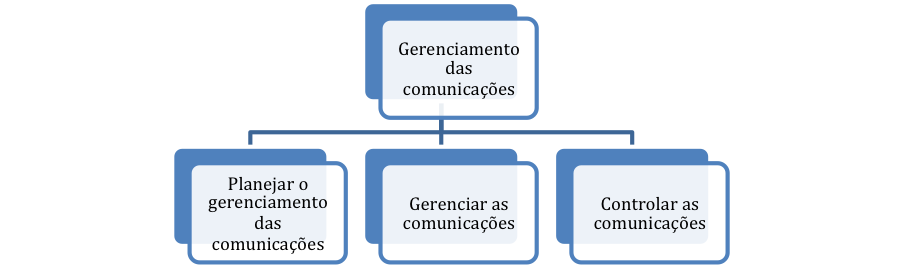
\includegraphics[scale=0.75]{Figuras/gerenciamento_comunicacoes.png}
	\caption{Processos do Gerenciamento das comunicações}
	\label{fig:proc:ger:comunic}
\end{figure}

\chapter{Planejar gerenciamento das comunicações}

O plano de gerenciamento das comunicações é o processo de desenvolver uma aproximação apropriada e um plano para as comunicações do projeto baseado nas necessidades e requisitos de informações das partes interessadas e nos ativos organizacionais disponíveis.

O processo de planejar o gerenciamento das comunicações está representado na Figura \ref{fig:comunic:plan:efts} e será descrito a seguir.

\begin{figure}[!h]
	\centering
	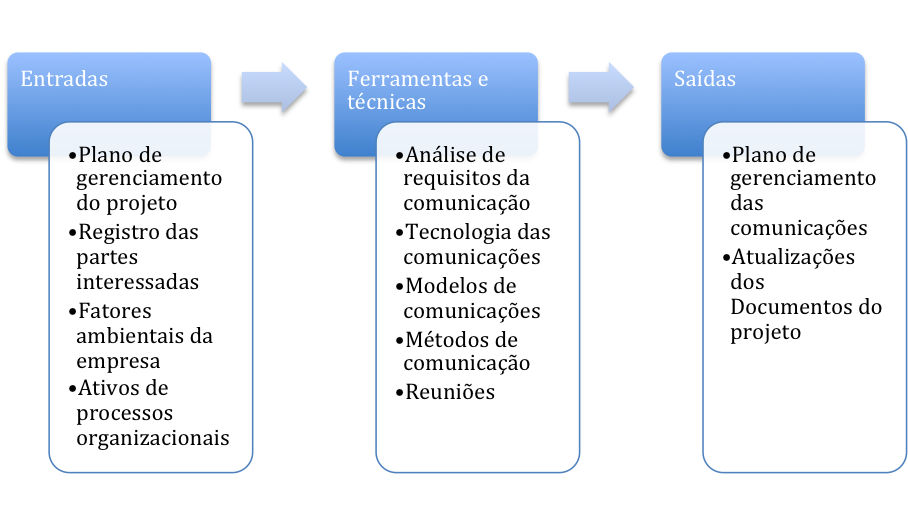
\includegraphics[scale=0.5]{Figuras/comunicacoes_efts_planejar.png}
	\caption{Planejar o gerenciamento das comunicações: entradas, ferramentas, técnicas e saídas}
	\label{fig:comunic:plan:efts}
\end{figure}

\section{Entradas}

\begin{description}
	
	\item[Plano de gerenciamento do projeto:] contém informações importantes para se executar, monitorar, controlar e encerrar o projeto.

	\item[Registro das partes interessadas:] contém necessidades e requisitos das partes interessadas.

	\item[Fatores ambientais da empresa:] intimamente ligado às comunicações, visto que a estrutura da organização terá um grande efeito nos requisitos das comunicações do projeto.

	\item[Ativos de processos organizacionais:] principalmente informações históricas e lições aprendidas, para avaliar as decisões tomadas sobre as comunicações e seus resultados.

\end{description}

\section{Ferramentas e técnicas}

\begin{description}

	\item[Análise de requisitos da comunicação:] determina a informação que as partes interessadas necessitam. Os requisitos são definidos pela combinação do tipo e formato da informação necessária através da análise do valor dessa informação.
	
	\item[Tecnologia das comunicações:] podem variar de acordo com a urgência da necessidade da informação, disponibilidade da tecnologia, facilidade de utilização, ambiente do projeto e sensibilidade e confiabilidade da informação.
	
	\item[Modelos de comunicações:] basicamente consiste no transmissor, receptor e meio. O transmissor é responsável pela tramissão da mensagem, pela garantia que a informação comunicada é clara e completa e pela confirmação que a comunicação foi corretamente entendida. O receptor é responsável por garantir que a informação foi recebida em sua totalidade, entendida corretamente e reconhecida ou respondida apropriadamente.
	
	\item[Métodos de comunicação:] de modo geral, são classifcadas em:
	
		\begin{description}
			
			\item[Comunicação interativa:] entre duas ou mais partes que estão realizando uma troca de informações multidirecional. É a forma mais eficiente de garantir um entendimento comum por todos os participantes sobre determinados tópicos. Inclui reuniões, telefonemas, videoconferências, etc.
			
			\item[Comunicação ativa (push):] encaminhada para destinatários específicos que precisam saber das informações. Garante que as informações sejam distribuídas mas não verifica se chegaram ou foram compreendidas pelo público-alvo. A comunicação ativa inclui cartas, memorandos, relatórios, emails, faxes, correio de voz, comunicados de imprensa, etc.
			
			\item[Comunicação passiva (pull):] usada para volumes muito grandes de informações ou para um público muito grande, requer que os destinatários acessem o conteúdo da comunicação a seu próprio critério. Esses métodos incluem sites de intranet, e-learning, repositórios de conhecimentos, etc.

		\end{description}	
		
	\item[Reuniões:] o planejamento do gerenciamento das comunicações requer discussões e diálogos com a equipe do projeto para determinar a forma mais apropriada de atualizar e comunicar as informações do projeto. Geralmente as reuniões facilitam essas discussões e diálogos.
	
\end{description}

\section{Saídas}

\begin{description}
	
	\item[Plano de gerenciamento das comunicações:] componente do \planproj que descreve como as comunicações do projeto serão planejadas, estruturadas, monitoradas e controladas.
	
	\item[Atualizações dos Documentos do projeto:] cronograma, registro de partes interessadas, etc.
	
\end{description}

\chapter{Gerenciar as comunicações}

Processo de criar, coletar, distribuir, armazenar, recuperar e disponibilizar as informações do projeto de acordo com o plano de gerenciamento das comunicações.

O processo de gerenciar as comunicações está representado na Figura \ref{fig:comunic:ger:efts} e será descrito a seguir.

\begin{figure}[!h]
	\centering
	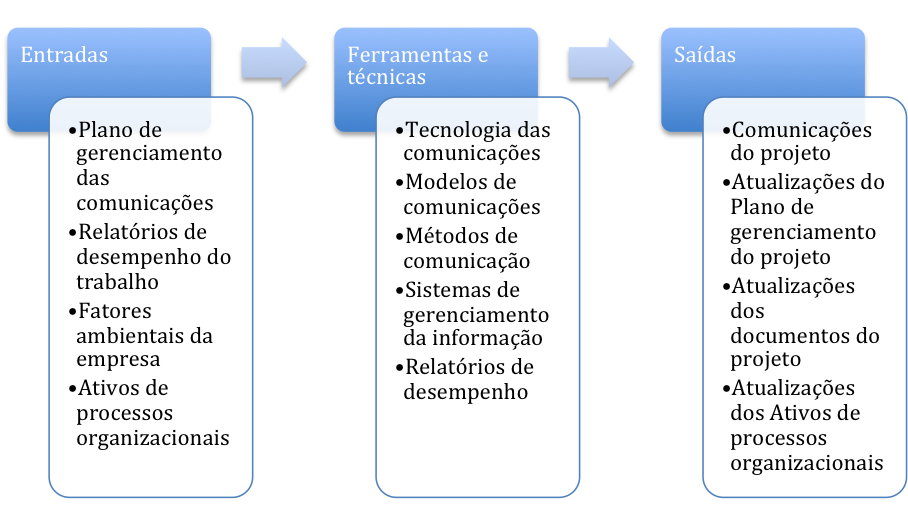
\includegraphics[scale=0.5]{Figuras/comunicacoes_efts_gerenciar.png}
	\caption{Gerenciar as comunicações: entradas, ferramentas, técnicas e saídas}
	\label{fig:comunic:ger:efts}
\end{figure}

\section{Entradas}

\begin{description}

	\item[Plano de gerenciamento das comunicações:] descreve como as comunicações do projeto serão planejadas, estruturadas, monitoradas e controladas.
	
	\item[Relatórios de desempenho do trabalho:] coleção de informações de performance e status do projeto que podem ser usadas para facilitar a discussão e criação das comunicações.
	
	\item[Fatores ambientais da empresa:] cultura e estrutura organizacional, padrões e regulamentações governamentais ou da indústria, sistemas de informação de gerência de projeto, etc.
	
	\item[Ativos de processos organizacionais:] políticas, procedimentos, processos e guias de gerenciamento de comunicações, modelos e informações históricas e lições aprendidas.

	
\end{description}

\section{Ferramentas e técnicas}

\begin{description}
	
	\item[Tecnologia das comunicações:] o foco é assegurar que a escolha seja apropriada para a informação que está sendo comunicada.
	
	\item[Modelos de comunicações:] o foco é assegurar que a escolha seja apropriada para o projeto e que barreiras (ruídos) sejam identificados e gerenciados.
	
	\item[Métodos de comunicação:] o foco é assegurar que a informação que foi criada e distribuída tenha sido recebida e compreendida para permitir resposta e feedback.
	
	\item[Sistemas de gerenciamento da informação:] ferramentas para gerenciar e distribuir informações do projeto.
	
	\item[Relatórios de desempenho:] ato de coletar e distribuir informações de desempenho, incluindo relatórios de status, medidads de progresso e previsões.
	
	
\end{description}

\section{Saídas}

\begin{description}
	
	\item[Comunicações do projeto:] relatórios de desempenho, status de entregas, progresso do cronograma, custos incorridos, etc.
	
	\item[Atualizações do Plano de gerenciamento do projeto:] o desempenho do projeto pode requerer alterações nas linhas de base do projeto.
	
	\item[Atualizações dos documentos do projeto:] o desempenho do projeto pode requerer alterações nos documentos do projeto.
	
	\item[Atualizações dos Ativos de processos organizacionais:] notificações de partes interessadas, relatórios do projeto, apresentações do projeto, registros do projeto, feedback das partes interessadas, lições aprendidas, etc.


\end{description}

\chapter{Controlar as comunicações}

Processo de monitorar e controlar as comunicações durante todo o ciclo de vida do projeto para garantir que as necessidades de informações das partes interessadas do projeto sejam satisfeitas.

O processo de controlar as comunicações está representado na Figura \ref{fig:comunic:controlar:efts} e será descrito a seguir.

\begin{figure}[!h]
	\centering
	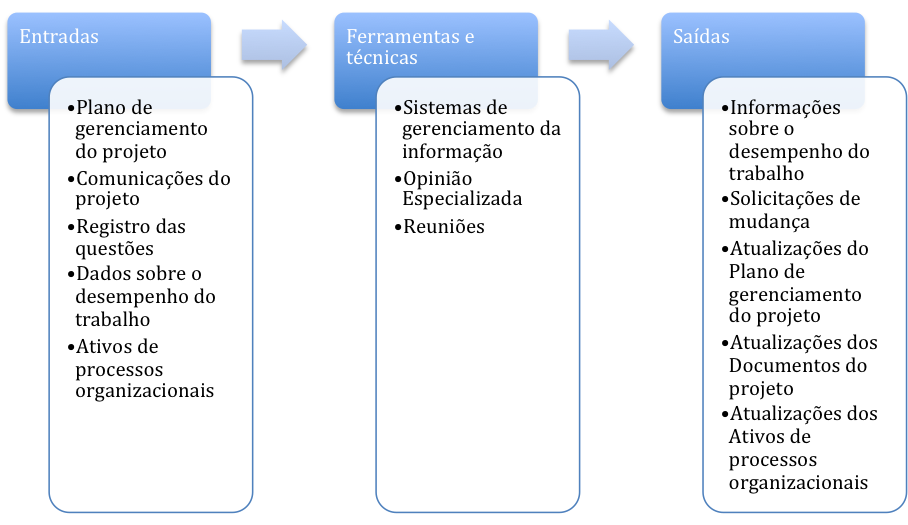
\includegraphics[scale=0.5]{Figuras/comunicacoes_efts_controlar.png}
	\caption{Controlar as comunicações: entradas, ferramentas, técnicas e saídas}
	\label{fig:comunic:controlar:efts}
\end{figure}

\section{Entradas}

\begin{description}

	\item[Plano de gerenciamento do projeto:] fornece os requisitos de comunicação das partes interessadas, razões para distruição das informações, tempo e frequência da distribuição das informações necessárias, responsáveis pelas comunicações das informações e receptores das informações.
	
	\item[Comunicações do projeto:] status das entregas, progresso do cronograma, custos incorridos, etc.
	
	\item[Registro das questões:] utilizado para documentar e monitorar a solução das questões.
	
	\item[Dados sobre o desempenho do trabalho:] detalhes sobre quais comunicações foram realmente distribuídas, feedbacks, pesquisas sobre efetividade das comunicações, etc.
	
	\item[Ativos de processos organizacionais:] modelos de relatórios, políticas, padrões e procedimentos que definem as comunicações, tecnologias disponíveis para comunicação, meios de comunicação permitidos, políticas de retenção de registros, requisitos de segurança, etc.
	
	
\end{description}

\section{Ferramentas e técnicas}

\begin{description}
	
	\item[Sistemas de gerenciamento da informação:] oferecem um conjunto de ferramentas padrão para o gerente de projetos capturar, armazenar e distribuir informações para as partes interessadas sobre os custos, cronograma e desempenho do projeto.
	
	\item[Opinião Especializada:] pode ser aplicada para detalhes técnicos e/ou gerenciais relativos às comunicações.
	
	\item[Reuniões:] facilitadoras de discussões e diálogos com a equipe de projeto que precisam determinar a forma mais apropriada de atualizar e comunicar o desempenho do projeto e responder às requisições de informações das partes interessadas.
	

\end{description}

\section{Saídas}

\begin{description}
	
	\item[Informações sobre o desempenho do trabalho:] organiza e sintetiza os dados de performance recolhidos.
	
	\item[Solicitações de mudança:] o processo de controle das comunicações geralmente resulta na necessidade de ajustes, ações e intervenções que, consequentemente, geram solicitações de mudanças.
	
	\item[Atualizações do Plano de gerenciamento do projeto:] planos de gerenciamento das partes interessadas e de recursos humanos, entre outros.
	
	\item[Atualizações dos Documentos do projeto:] previsões, relatórios de desempenho de trabalho, registro de questões, etc.
	
	\item[Atualizações dos Ativos de processos organizacionais:] formato de relatórios, documentação das lições aprendidas, etc.
	
\end{description}